\newpage
\section{E-Mails und deren Tücken}
Täglich werden heute bis zu 180 Milliarden E-Mails pro Tag versendet. Eine gewaltige Menge, wenn man bedenkt, dass es ein wenig mehr als sieben Milliarden Menschen auf diesem Planet gibt.
Doch nur wenige E-Mail Nutzer machen sich Gedanken darüber, was denn eigentlich hinter einer E-Mail steckt. Wohin geht sie genau? Wer alles kann diese E-Mail theoretisch lesen? Wo wird diese Nachricht, wenn ich sie mal versendet habe, überall gespeichert? Und für wie lange? Gibt es Kopien? Backups? Auf anderen Servern?
All diese Fragen sind sehr wichtig, wenn man vertrauliche Daten per Mail versendet. Aber nicht nur dann, denn selbst wenn die Nachricht nicht von grosser Bedeutung ist, so möchte man doch eine gewisse Privatsphäre wahren.
Was kann man also als „0815“ Privatbenutzer einer E-Mail Adresse tun um seine eigenen Mails möglichst sicher zu versenden, zu speichern und  zu empfangen?
Im nächsten Kapitel wird versucht auf alle diese Fragen eine Antwort zu finden. Zuerst einmal muss man aber verstehen, wie das genau funktioniert, mit den „Mails“.

\subsection{Funktionsweise des Mailverkehrs}
Das Erste was wir wohl tun werden, nach dem wir den Entschluss gefällt haben eine E-Mail versenden zu wollen, ist es unseren Computer zu starten und unseren E-Mail Client aufzumachen. Ein solcher Client kann etwa Mozilla Thunderbird, Apple Mail oder Microsoft Outlook sein. Traditionellerweise gehen wir davon aus, dass unser Client mindestens mit den Funktionen um eine E-Mail zu versenden und zu empfangen ausgestattet ist.
Wir haben nun unsere E-Mail verfasst und drücken in unserem Client auf den „Senden“ Knopf. Was passiert nun mit der Mail?
Diese wird, sofern eine Verbindung ins Internet besteht, zum konfigurierten SMTP-Server gesendet. Ein SMTP-Server ist ein Computer im Internet, der die Aufgabe hat, eine E-Mail zum Empfänger zu transportieren. Man nennt einen solchen Server deshalb „Mail Transport Agent“ kurz MTA. Sobald dieser Server den Empfänger ausfindig machen konnte, wird die E-Mail an den MTA des Empfängers weitergeleitet. Dort angekomment legt dieser MTA die E-Mail beim „Mail Delivery Agent“ kurz MDA des Empfängers ab.
Auf der anderen Seite gibt es nun natürlich auch den Empfänger, welcher auch einen Computer mit E-Mail Client hat und gerne die Nachricht, die wir ihm anfangs zukommen lassen hatten, lesen möchte. Wie schon erwähnt hat so ein „traditioneller“ Client auch die Funktion Mails empfangen zu können. Dazu wird analog zum SMTP-Server des Senders auch ein Server konfiguriert um Mails von seinem Postfach abrufen zu können. Dieser Server, der die Funktion der MDA hat, nennt man POP- oder IMAP-Server. Zwischen diesen beiden Arten von Mail Delivery Agents gibt es einen grossen und nützlichen Unterschied, denn im Gegensatz zum POP-Server kann der IMAP-Server die Mails zwischen mehreren Clients synchronisieren, dazu gehört etwa ein Status, ob die Mail schon gelesen oder als wichtig markiert wurde. So wird natürlich beim IMAP-Server auch immer, aus Synchronisationsgründen, eine Kopie der Nachricht auf dem Server belassen, wohingegen diese Option bei einem POP-Server nicht gesetzt sein muss.
So will nun also unser Empfänger die Mails seines Postfachs lesen. Dazu verbindet sich, wie schon gesagt, der E-Mail Client mit dem konfigurieren MDA. Dieser MDA kann nun die Nachricht, die er vom Transport Agent bekommen hat dem Empfänger zurückschicken.
\footnote{\url{http://de.wikipedia.org/wiki/Mail_Delivery_Agent}}
\footnote{\url{http://de.wikipedia.org/wiki/Mail_Transport_Agent}}
\\

\begin{figure}
\centering
\noindent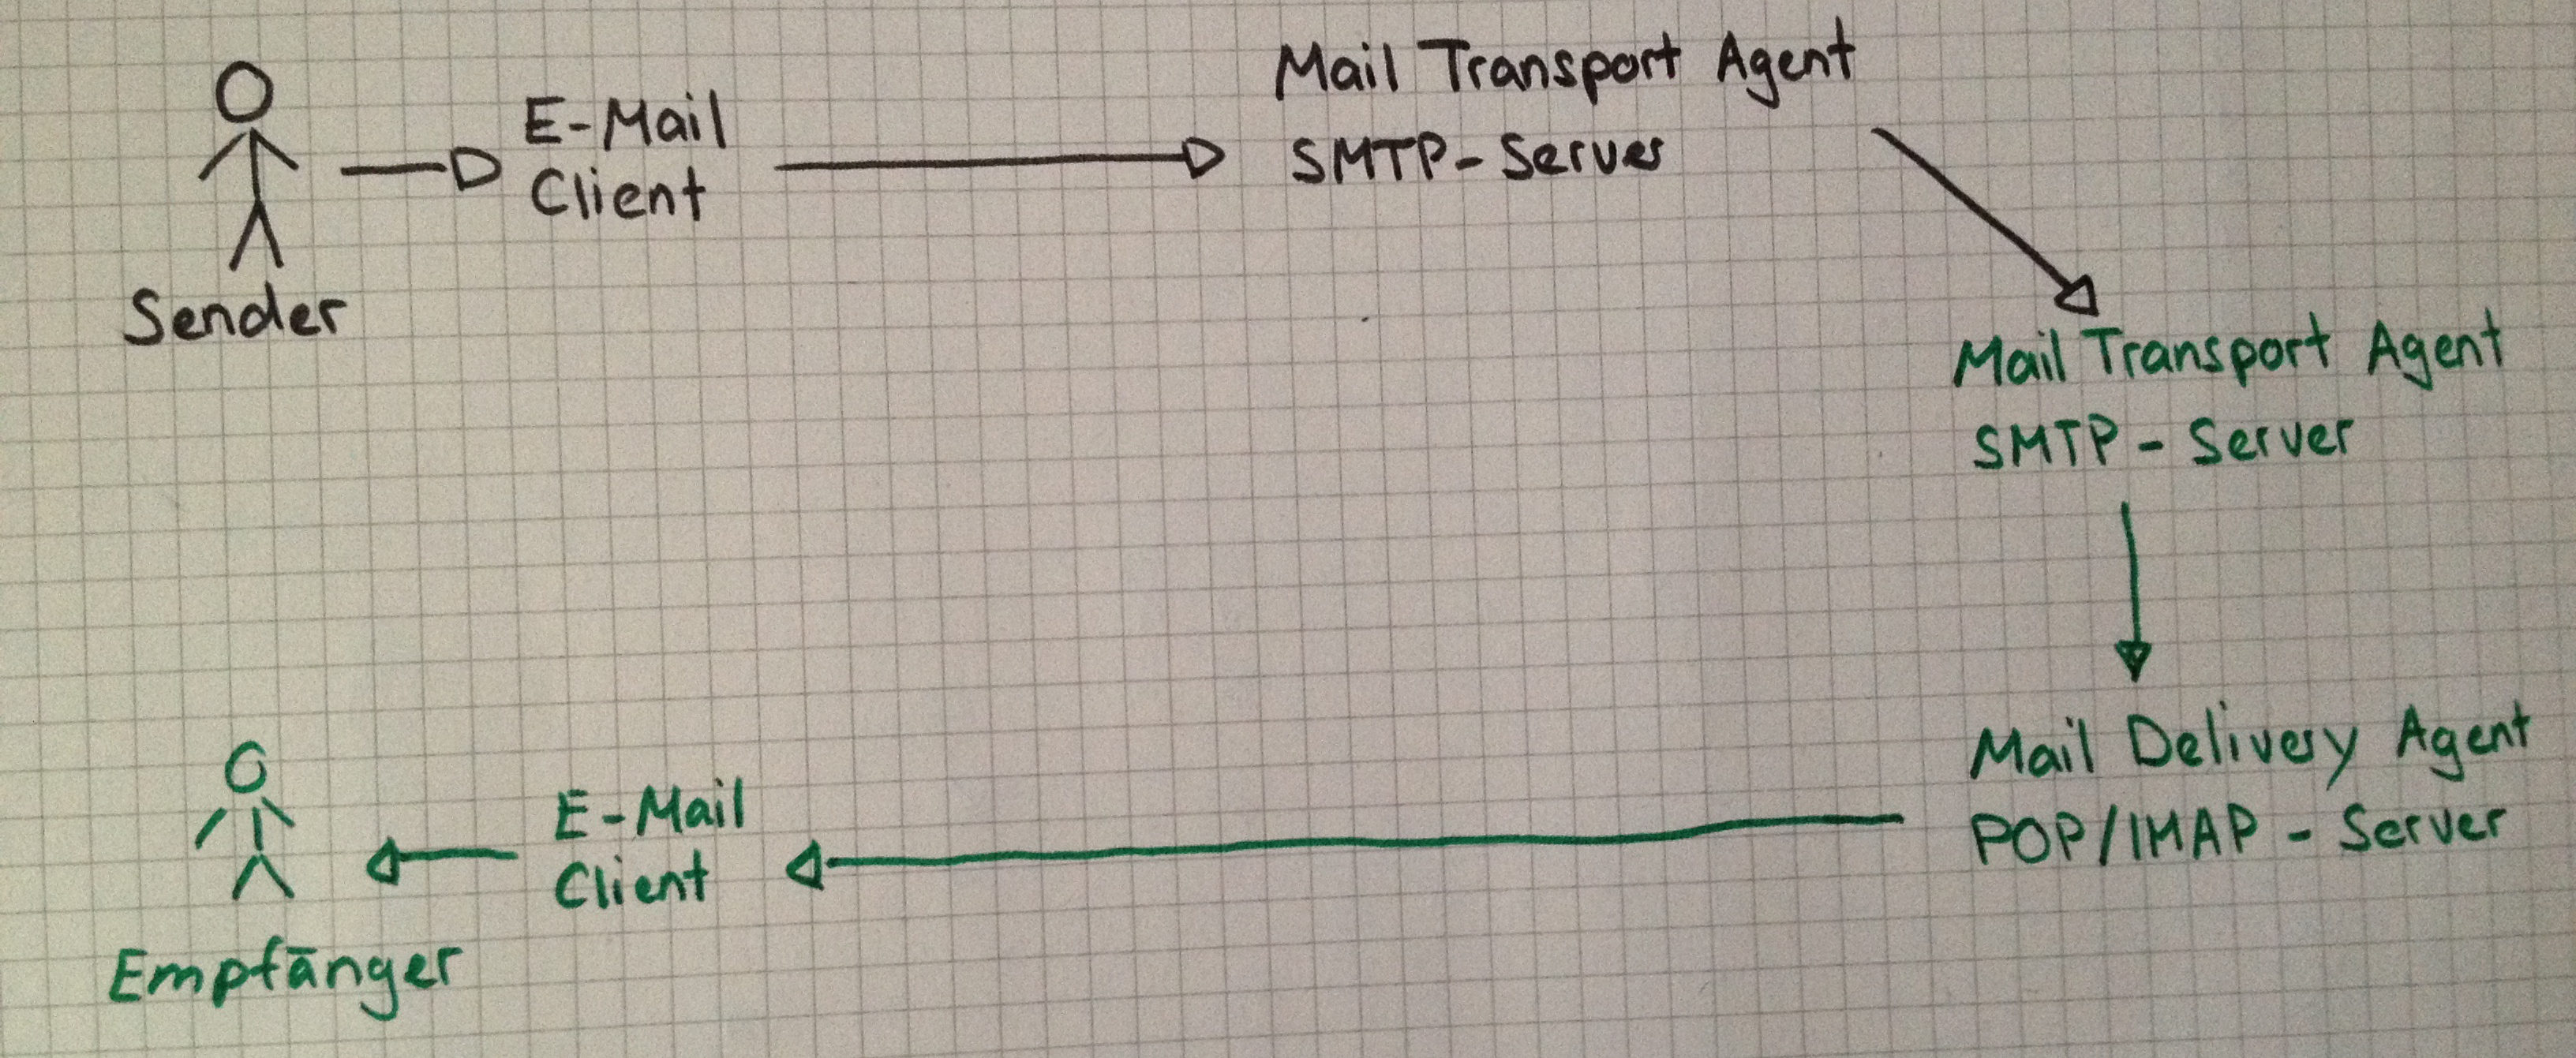
\includegraphics[scale=0.14]{images/mailverkehr.jpg}
\caption{Funktionsweise Mailverkehr}
\end{figure}


\subsection{Mein Provider und seine Server}
Die erste Entscheidung, die man treffen muss, um überhaupt eine E-Mail senden zu können, noch bevor man überhautp seinen Mail-Client startet, ist es, sich einen passenden Provider auszusuchen. Ein Provider ist meist eine Firma, die seinen Kunden eine Mail Adresse zur Verfügung stellt. Dies kann z.B. Google mit Gmail, Microsoft mit Hotmail oder eine Firma wie GMX sein. Was ein solcher Provider also tut, ist es irgendwo eine E-Mail Adresse für den Kunden zu konfigurieren. Dazu gehört einmal eine Adresse zum Mail Transport Agent und eine Adresse zum Mail Delivery Agent Server.
Diese beiden Server sind nicht nur auf den Bezug für die Mailfunktionalität im allgemeinen von Bedeutung. Nein, denn dort, auf diesen Servern, unter der Kontrolle des jeweiligen Providers, geht jede einzelne E-Mail, die versendet oder empfangen wird durch, was bedeutet, dass dort theoretisch ein Mitschnitt aller Nachrichten gemacht werden kann. Auch macht der Provider, natürlich nur zum besten seiner Kunden, Backups deren Postfächer, auf dem MDA. Das mag ja schön und gut sein, aber wer, ausser meinerselbst kann auch noch auf dieses Postfach oder die Backup-Daten zugreifen? Die Systemadministratoren vom Provider? PR-Firmen? Datenanalysten? Geheimdienste? Wer weiss …
Wie man sehen kann, hat man, abgesehen vom Vertrauen, im Prinzip keine Ahnung, wer alles auf seine E-Mails zugreifen kann.
\subsection{E-Mails verschlüsseln}
Doch es gibt ein paar Dinge, die man als E-Mail Nutzer tun kann, um seine Post einigermassen vor ungewollten Blicken schützen zu können.
So gibt es mehrere Verfahren um E-Mails zu verschlüsseln. Eines der beliebtesten und wohl meist verbreitesten ist PGP (Pretty Good Privacy) oder deren Weiterentwicklung GPG (GNU Privacy Guard).
Bei beiden handelt es sich um ein Public-Key-Verfahren mit asymmetrischer Verschlüsselung. Das heisst, dass es einmal einen öffentlichen Schlüssel gibt, mit dem jeder beliebige Daten für den Empfänger verschlüsseln und signieren kann und einen privaten geheimen Schlüssel der vom Empfänger benutzt wird um die Nachricht, die mit seinem öffentlichen Schlüssel verschlüsselt wurde, zu entschlüsseln.
Solange man seinen privaten Schlüssel geheim behält, ist es wahnsinnig schwierig, sowie sehr Rechenleistungs- und Zeitinsensiv einen solch verschlüsselte Nachricht zu knacken.
Es gibt eine Menge an Erweiterungen für die gängisten Mail-Clients um diese Verschlüsselungsfunktion nach zu rüsten.
\subsection{Ich als Provider}
Wie wir gesehen haben, macht ein Provider eigentlich nicht viel aus. Was dieser lediglich zu tun hat, damit man E-Mails versenden und empfangen kann, ist es einen MTA und einen MDA zur Verfügung zu stellen, sowie die E-Mail Adresse korrekt zu konfigureren, damit die Mails auch ihren richtigen Weg gehen. Natürlich müssen diese beiden Server am Internet angehängt sein und dauerhaft laufen.
Jeder E-Mail Provider hat zudem seine eigene Domain, wie zum Beispiel Google's \textit{gmail.com} oder Swisscom's \textit{bluewin.ch}. Die Kunden E-Mail Adressen enden also immer auf jene Domains: \textit{max@gmail.com}, \textit{muster@bluewin.ch}. Natürlich braucht man auch selbst eine solche Domain. Diese muss nicht zwingend eine Top-Level-Domain \footnote{\url{http://de.wikipedia.org/wiki/Top-Level-Domain}} sein. Auch eine kostenlose Domain mit der Endung \textit{.ch.vu} würde genügen. Dieser Domain braucht man dann nur noch einen DNS-Server \footnote{\url{http://de.wikipedia.org/wiki/Domain\_Name\_System}} zuweisen, der unsere MDA Server IP kennt. Ein Problem gibt es da aber noch und zwar, dass normale Haushaulte vom Internetprovider keine statische IP Adresse bekommen, was bedeutet, dass diese ständig ändern könnte und so der DNS-Server nicht mehr weiss wohin er jetzt den Datenverkehr weiterleiten muss. Hier gibt es zwei Lösungen, um dieses Problem zu vermeiden: Man kann beim Provider eine meist kostenpflichtige statische IP Adresse verlangen oder man registriert sich bei einem dynamischen DNS Anbieter. Dieser bietet eine Schnittstelle zur Verfügung, über die man seine Server IP Adresse, immer wenn diese ändert, dem DNS mitteilen kann. Somit ist gegeben, dass der DNS Server stets die aktuelle IP Adresse des Servers kennt ohne dass man auf eine kostenpflichtige statische IP Adresse zurückgreifen muss.

\subsection{Vor- und Nachteile}
Natürlich gibt es nicht nur Vorteile wenn man sein eigener E-Mail Provider ist. Folgende Auflistung soll hier eine Übersicht schaffen. \\ \\

\textbf{Vorteile:}
\begin{itemize}
    \item Volle Kontrolle
    \item Verschlüsselung
\end{itemize}

\textbf{Nachteile:}
\begin{itemize}
    \item Hardware- und Unterhaltungs-Kosten
    \item Benötigte Zeit
\end{itemize}
